\chapter{Specifikacija programske potpore}
		
	\section{Funkcionalni zahtjevi}
			
			\noindent \textbf{Dionici:}
			
			\begin{packed_enum}
				
				\item Registrirani korisnik/Ponuditelj		
				\item Strani izdavač
                \item Izdavač
                \item Antikvarijat
                \item Preprodavač
                \item Razvojni tim
    
			\end{packed_enum}
			
			\noindent \textbf{Aktori i njihovi funkcionalni zahtjevi:}
			
			
			\begin{packed_enum}
				\item  \underbar{Neregistrirani korisnik(inicijator) može:}
				
				\begin{packed_enum}
					
					\item Pretraživati knjige po njihovim atributima
					\item Pretraživati na karti izdavače
                    \item Pretraživati izdavače po imenu
                    \item Tražiti strane izdavače da se knjiga prevede
					%\begin{packed_enum}
						
						%\item  podfunkcionalnost 1 
						%\item  podfunkcionalnost 2
				
					%\end{packed_enum}
		
				\end{packed_enum}
			
				\item  \underbar{Registrirani korisnik(izdavač/antikvarijat/preprodavač)(inicijator) može:}
				
				\begin{packed_enum}
					
					\item Stavljati objave za knjige
					\item Mijenjati objave za knjige
                    \item Brisati objave za knjige
                    \item Tražiti stranog izdavača za prijevod knjige
                    \item Birati u koju kategoriju ponuditelja će spadati
					
				\end{packed_enum}

                \item \underbar{Administrator(sudionik):}
                \begin{packed_enum}
                    \item Prima zahtjev za registraciju i na temelju unesenih podataka potvrđuje ili odbija registraciju
                \end{packed_enum}

                \item \underbar{Strani izdavač(sudionik):}
                \begin{packed_enum}
                    \item Prima zahtjev od strane izdavača za prijevod knjige
                \end{packed_enum}

                \item \underbar{Baza podataka(sudionik):}
                \begin{packed_enum}
                    \item Pohranjuje podatke o korisnicima i njihovim ovlastima
                    \item Pohranjuje podatke o objavljenim knjigama
                \end{packed_enum}
			\end{packed_enum}
			
			\eject 
			
			
			\subsection{Obrasci uporabe}
				

				
				\subsubsection{Opis obrazaca uporabe}				
					\noindent \underbar{\textbf{UC1 - Registracija}}
					\begin{packed_item}
	
						\item \textbf{Glavni sudionik: } Ponuditelj
						\item  \textbf{Cilj:} Izrada korisničkog računa za web stranicu
						\item  \textbf{Sudionici:} Baza podataka
						\item  \textbf{Preduvjet:} -
						\item  \textbf{Opis osnovnog tijeka:}
						
						\item[] \begin{packed_enum}
	
							\item Ponuditelj bira opciju registracije
                            \item Ponuditelj unosi podatke potrebne za registraciju
							\item Web obavještava ponuditelja da je registracija uspješna
						\end{packed_enum}
						
						\item  \textbf{Opis mogućih odstupanja:}
						
						\item[] \begin{packed_item}
	
							\item[2.a] Ponuditelj unosi zauzeto korisničko ime, e-mail ili broj telefona ili je neki od podataka u krivom formatu
							\item[] \begin{packed_enum}
								
								\item Sustav obavještava o neuspjeloj registraciji i gdje je došlo do greške
								\item Ponuditelj unosi prihvatljive podatke ili odustane od registracije
								
							\end{packed_enum}
						\end{packed_item}
					\end{packed_item}

                    \noindent \underbar{\textbf{UC2- Prijava}}
					\begin{packed_item}
	
						\item \textbf{Glavni sudionik: } Ponuditelj
						\item  \textbf{Cilj:} Dobiti pristup web stranici sa postojećim korisničkim računom
						\item  \textbf{Sudionici:} Baza podataka
						\item  \textbf{Preduvjet:} - Ponuditelj ima izrađen korisnički račun
						\item  \textbf{Opis osnovnog tijeka:}
						
						\item[] \begin{packed_enum}
	
							\item Ponuditelj bira opciju prijave
							\item Ponuditelj unosi korisničko ime i lozinku
                            \item Ponuditelj dobiva pristup svom korisničkom računu
						\end{packed_enum}
						
						\item  \textbf{Opis mogućih odstupanja:}
						
						\item[] \begin{packed_item}
	
							\item[2.a] Jedan ili više potrebnih podataka je krivo uneseno
							\item[] \begin{packed_enum}
								
								\item Sustav obavještava o neuspjeloj prijavi i gdje je došlo do greške
								\item Ponuditelj unosi prihvatljive podatke ili odustane od prijave
								
							\end{packed_enum}
						\end{packed_item}
					\end{packed_item}

                    \noindent \underbar{\textbf{UC3 - Potvrda registracije}}
					\begin{packed_item}
	
						\item \textbf{Glavni sudionik: } Administrator
						\item  \textbf{Cilj:} Potvrđivanje uspješne/neuspješne registracije ponuditelja
						\item  \textbf{Sudionici:} Baza podataka, Ponuditelj
						\item  \textbf{Preduvjet:} - Ponuditelj pokušava izvršiti registraciju
						\item  \textbf{Opis osnovnog tijeka:}
						
						\item[] \begin{packed_enum}
	
							\item Nakon što ponuditelj unese podatke za registraciju, zahtjev za registraciju se šalje administratoru na pregled
							\item Provjerava se da su uneseni podaci dobrog oblika i da ne postoje u bazi podataka
                            \item Administrator potvrđuje unesene podatke i informira da je registracija uspješna
						\end{packed_enum}
						
						\item  \textbf{Opis mogućih odstupanja:}
						
						\item[] \begin{packed_item}
	
							\item[2.a] Podaci su krivog formata ili već upisani u bazu podataka jer ih netko drugi koristi
							\item[] \begin{packed_enum}			
								\item Administrator obavještava da je došlo do greške i zašto
							\end{packed_enum}
						\end{packed_item}
					\end{packed_item}

                    \noindent \underbar{\textbf{UC4 - Biranje kategorije ponuditelja}}
					\begin{packed_item}
	
						\item \textbf{Glavni sudionik: } Ponuditelj
						\item  \textbf{Cilj:} Biranje kategorije ponuditelja u koju će spadati korisnički račun
						\item  \textbf{Sudionici:} Baza podataka
						\item  \textbf{Preduvjet:} - Pondutelj je započeo registraciju
						\item  \textbf{Opis osnovnog tijeka:}
						
						\item[] \begin{packed_enum}
	
							\item Pri registraciji ponuditelj klikne na polje kojim bira u koju će kategoriju spadati
							\item Ponuditelja bira kategoriju i nastavlja sa registracijom
						\end{packed_enum}
						
						\item  \textbf{Opis mogućih odstupanja:-}
					
					\end{packed_item}

                    \noindent \underbar{\textbf{UC5 - Pregled korisničkog računa}}
					\begin{packed_item}
	
						\item \textbf{Glavni sudionik: } Ponuditelj
						\item  \textbf{Cilj:} Ponuditelj pregledava podatke o svom korisničkom računu
						\item  \textbf{Sudionici:} Baza podataka
						\item  \textbf{Preduvjet:} - Ponuditelj je prijavljen
						\item  \textbf{Opis osnovnog tijeka:}
						
						\item[] \begin{packed_enum}
	
							\item Ponuditelj bira opciju "Moj račun"
							\item Aplikacija prikazuje pripadni korisnički račun i podatke
						\end{packed_enum}
						
						\item  \textbf{Opis mogućih odstupanja: -}
						
					\end{packed_item}

                    \noindent \underbar{\textbf{UC6 - Promjena podataka}}
					\begin{packed_item}
	
						\item \textbf{Glavni sudionik: } Ponuditelj
						\item  \textbf{Cilj:} Ponuditelj mijenja podatke svog korisničkog računa
						\item  \textbf{Sudionici:} Baza podataka
						\item  \textbf{Preduvjet:} - Ponuditelj je prijavljen
						\item  \textbf{Opis osnovnog tijeka:}
						
						\item[] \begin{packed_enum}
	
							\item Ponuditelj bira opciju "Moj račun"
							\item Ponuditelj bira opciju "Uredi račun"
                            \item Ponuditelj mijenja podatke
                            \item Ponuditelj sprema izmjene
                            \item Baza podataka se ažurira
						\end{packed_enum}
						
						\item  \textbf{Opis mogućih odstupanja:}
						
						\item[] \begin{packed_item}
	
							\item[2.a] Ponuditelj unosi podatke u krivom formatu ili su podaci već korišteni od strane drugih ponuditelja
							\item[] \begin{packed_enum}
								
								\item Aplikacija obavještava da je došlo do greške i zašto
								\item Ponuditelj opet pokušava promjeniti podatke ili odustaje
							\end{packed_enum}

                            \item[2.b] Ponuditelj upisuje nove podatke ali ne klikne na opciju spremanja promjena
                            \item[] \begin{packed_enum}
                                \item Aplikacija obavještava da promjene nisu pohranjene
                            \end{packed_enum}
						\end{packed_item}
					\end{packed_item}

                    \noindent \underbar{\textbf{UC7 - Brisanje korisničkog računa}}
					\begin{packed_item}
	
						\item \textbf{Glavni sudionik: } Ponuditelj
						\item  \textbf{Cilj:} Ponuditelj briše svoj račun sa web stranice
						\item  \textbf{Sudionici:} Baza podataka
						\item  \textbf{Preduvjet:} - Ponuditelj ima izrađen korisnički račun
						\item  \textbf{Opis osnovnog tijeka:}
						
						\item[] \begin{packed_enum}
	
							\item Ponuditelj bira opciju "Moj račun"
                            \item Ponuditelj bira opciju brisanja korisničkog računa
							\item Aplikacija traži potvrdu brisanja
                            \item Ponuditelj potvrđuje brisanje korisničkog računa
                            \item Miču se podaci o računu iz baze podataka
                            \item Ponuditelj je vraćen na stranicu za upis
						\end{packed_enum}
						
						\item  \textbf{Opis mogućih odstupanja: -}
					\end{packed_item}

                    \noindent \underbar{\textbf{UC8 - Dodavane objave knjige}}
					\begin{packed_item}
	
						\item \textbf{Glavni sudionik: } Ponuditelj
						\item  \textbf{Cilj:} Dodavanje objave knjige za prodaju na web stranicu
						\item  \textbf{Sudionici:} Baza podataka
						\item  \textbf{Preduvjet:} - Ponuditelj je prijavljen
						\item  \textbf{Opis osnovnog tijeka:}
						
						\item[] \begin{packed_enum}
	
							\item Ponuditelj bira opciju "Nova objava"
                            \item Aplikacija otvara stranicu za novu objavu
                            \item Ponuditelj unosi potrebne podatke
							\item Ponuditelj klikne opciju "Objavi"
                            \item Objava knjige je vidljiva na web stranici i u bazi podataka
						\end{packed_enum}
						
						\item  \textbf{Opis mogućih odstupanja:}
						
						\item[] \begin{packed_item}
	
							\item[2.a] Ponuditelj unosi krivi format podataka potrebnih za objavu
							\item[] \begin{packed_enum}
								
								\item Aplikacija obavještava da je format kriv i gdje
								\item Ponuditelj unosi prihvatljive podatke ili odustaje od objave
							\end{packed_enum}
                            \item[2.b] Ponuditelj ne unosi sve potrebne podatke da se napravi objava
                             \item[] \begin{packed_enum}
                                 \item Aplikacija obavještava koje polje nije popunjeno
                                 \item Ponuditelj popunjuje prazna polja ili odustaje od objave
                             \end{packed_enum}
						\end{packed_item}
					\end{packed_item}

                    \noindent \underbar{\textbf{UC9 - Mijenjanje objave}}
					\begin{packed_item}
	
						\item \textbf{Glavni sudionik: } Ponuditelj
						\item  \textbf{Cilj:} Mijenjanje podataka objave za knjigu
						\item  \textbf{Sudionici:} Baza podataka
						\item  \textbf{Preduvjet:} - Postoji objava za knjigu
						\item  \textbf{Opis osnovnog tijeka:}
						
						\item[] \begin{packed_enum}
	
							\item Ponuditelj klikne na objavu koju želi promjeniti
                            \item Aplikacija otvara stranicu objave
							\item Ponuditelj bira opciju mijenjanja podataka
                            \item Ponuditelj izmjenjue podatke
                            \item Ponuditelj sprema izmjene
                            \item Novi podaci su zapisani u bazu podataka
						\end{packed_enum}
						
						\item  \textbf{Opis mogućih odstupanja:}
						
						\item[] \begin{packed_item}
	
							\item[2.a] Ponuditelj unosi podatke u krivom formatu
							\item[] \begin{packed_enum}
								
								\item Aplikacija obavještava gdje je došlo do greške i zašto
								\item Ponuditelj unosi prihvatljive podatke ili odustane od izmjene podataka
								
							\end{packed_enum}

                            \item[2.b] Ponuditelj ne sprema izmjene
                            \item[] \begin{packed_enum}

                                \item Aplikacija obavještava da promjene nisu pohranjene
                            \end{packed_enum}
						\end{packed_item}
					\end{packed_item}

                    \noindent \underbar{\textbf{UC10 - Brisanje objave}}
					\begin{packed_item}
	
						\item \textbf{Glavni sudionik: } Ponuditelj
						\item  \textbf{Cilj:} Ponuditelj briše svoju objavu
						\item  \textbf{Sudionici:} Baza podataka
						\item  \textbf{Preduvjet:} - Ponuditelj ima objavu
						\item  \textbf{Opis osnovnog tijeka:}
						
						\item[] \begin{packed_enum}
	
							\item Ponuditelj klikne na objavu koju želi izbrisati
                            \item Ponuditelj bira opciju brisanja objave
							\item Aplikacija pita za potvrdu brisanja
                            \item Ponuditelj potvrđuje
                            \item Briše se objava iz baze podataka
						\end{packed_enum}
						
						\item  \textbf{Opis mogućih odstupanja: -}
					\end{packed_item}

                    \noindent \underbar{\textbf{UC11 - Pregled objave}}
					\begin{packed_item}
	
						\item \textbf{Glavni sudionik: } Neregistrirani korisnik
						\item  \textbf{Cilj:} Izrada korisničkog računa za web stranicu
						\item  \textbf{Sudionici:} Baza podataka, Ponuditelj
						\item  \textbf{Preduvjet:} - Ponuditelj ima objavu knjige
						\item  \textbf{Opis osnovnog tijeka:}
						
						\item[] \begin{packed_enum}
	
							\item Neregistrirani korisnik klikne na objavu
                            \item Aplikacija prikazuje objavu i podatke o knjizi
						\end{packed_enum}
						
						\item  \textbf{Opis mogućih odstupanja: -}
					\end{packed_item}

                    \noindent \underbar{\textbf{UC12 - Pregled profila ponuditelja}}
					\begin{packed_item}
	
						\item \textbf{Glavni sudionik: } Neregistrirani korisnik
						\item  \textbf{Cilj:} Neregistrirani korisnik pregledava korisnički račun ponuditelja
						\item  \textbf{Sudionici:} Baza podataka
						\item  \textbf{Preduvjet:} - Ponuditelj ima izrađen korisnički račun
						\item  \textbf{Opis osnovnog tijeka:}
						
						\item[] \begin{packed_enum}
	
							\item Neregistrirani korisnik klikne na opciju pregledavanja računa ponuditelja
                            \item Aplikacija otvara stranicu na kojoj prikazuje podatke o računu ponuditelja
						\end{packed_enum}
						
						\item  \textbf{Opis mogućih odstupanja: -}
					\end{packed_item}

                    \noindent \underbar{\textbf{UC13 - Zahtjev da se prevede knjiga}}
					\begin{packed_item}
	
						\item \textbf{Glavni sudionik: } Neregistrirani korisnik
						\item  \textbf{Cilj:} Neregistrirani korisnik traži izdavača da se knjiga prevede
						\item  \textbf{Sudionici:} Baza podataka, izdavač
						\item  \textbf{Preduvjet:} - Postoji objava za knjigu
						\item  \textbf{Opis osnovnog tijeka:}
						
						\item[] \begin{packed_enum}
	
							\item Neregistrirani korisnik klikne na objavu za knjigu
                            \item Aplikacija otvara stranicu objave 
							\item Neregistrirani korisnik klikne na opciju "Zatraži prijevod knjige"
                            \item U bazi podataka se inkrementira broj zatraženih prijevoda za tu knjigu
						\end{packed_enum}
						
						\item  \textbf{Opis mogućih odstupanja: -}
					\end{packed_item}

                    \noindent \underbar{\textbf{UC14 - Zahtjev stranom izdavaču za prijevod knjige}}
					\begin{packed_item}
	
						\item \textbf{Glavni sudionik: } Izdavač
						\item  \textbf{Cilj:} Izrada korisničkog računa za web stranicu
						\item  \textbf{Sudionici:} Baza podataka, strani izdavač
						\item  \textbf{Preduvjet:} -
						\item  \textbf{Opis osnovnog tijeka:}
						
						\item[] \begin{packed_enum}
	
							\item Ponuditelj na svojoj objavi klikne opciju "Zatraži stranog izdavača za prijevod"
                            \item U bazi podataka se inkrementira broj zatraženih prijevoda od strane izdavača
						\end{packed_enum}
						
						\item  \textbf{Opis mogućih odstupanja: -}
					\end{packed_item}

                    \noindent \underbar{\textbf{UC15 - Pretraživanje po lokaciji}}
					\begin{packed_item}
	
						\item \textbf{Glavni sudionik: } Neregistrirani korisnik
						\item  \textbf{Cilj:} Pretraživanje ponuditelja na mapi koristeći objavljene lokacije
						\item  \textbf{Sudionici:} Baza podataka, ponuditelj
						\item  \textbf{Preduvjet:} - Ponuditelj ima objavljenu lokaciju
						\item  \textbf{Opis osnovnog tijeka:}
						
						\item[] \begin{packed_enum}
	
							\item Na glavnoj stranici je karta na kojoj se vide označene adrese ponuditelja
                            \item Neregistrirani korisnik može biranjem lokacije vidjeti ponuditelja/e koji se tamo nalaze
						\end{packed_enum}
						
						\item  \textbf{Opis mogućih odstupanja: -}
					\end{packed_item}

                    \noindent \underbar{\textbf{UC16 - Detaljna pretraga objava knjiga}}
					\begin{packed_item}
	
						\item \textbf{Glavni sudionik: } Neregistrirani korisnik
						\item  \textbf{Cilj:} Pretraživanje objava knjiga po atributima
						\item  \textbf{Sudionici:} Baza podataka
						\item  \textbf{Preduvjet:} - Postoji objava za traženu knjigu
						\item  \textbf{Opis osnovnog tijeka:}
						
						\item[] \begin{packed_enum}
	
							\item Neregistrirani korisnik klikne na opciju pretraživanja objava
                            \item NAPOMENA: daljnji koraci nisu obavezni, ali povećavaju vjerojatnost pronalaska tražene knjige
							\item Korisnik ispunjuje sljedeća polja: naziv knjige, naziv autora, godina izdanja, redni broj izdanja, kategorija izdavača, žanr knjige, ISBN, oznaka vrste knjige
						\end{packed_enum}
						
						\item  \textbf{Opis mogućih odstupanja: -}
					\end{packed_item}

                    \noindent \underbar{\textbf{UC17 - Pretraga ponuditelja}}
					\begin{packed_item}
	
						\item \textbf{Glavni sudionik: } Neregistrirani korisnik
						\item  \textbf{Cilj:} PPretraživanje ponuditelja sa korisničkim računom
						\item  \textbf{Sudionici:} Baza podataka, ponuditelj
						\item  \textbf{Preduvjet:} - Ponuditelj ima izrađen korisnički račun
						\item  \textbf{Opis osnovnog tijeka:}
						
						\item[] \begin{packed_enum}
	
							\item Neregistrirani korisnik bira opciju pretraživanja po ponuditeljima
                            \item Korisnik upisuje ime ponuditelja
							\item Aplikacija izbacuje rezultate koji se poklapaju
						\end{packed_enum}
						
						\item  \textbf{Opis mogućih odstupanja: -}
					\end{packed_item}
				
				\subsubsection{Dijagrami obrazaca uporabe}
					
Dijagram obrazaca 1

\begin{figure}
    \centering
    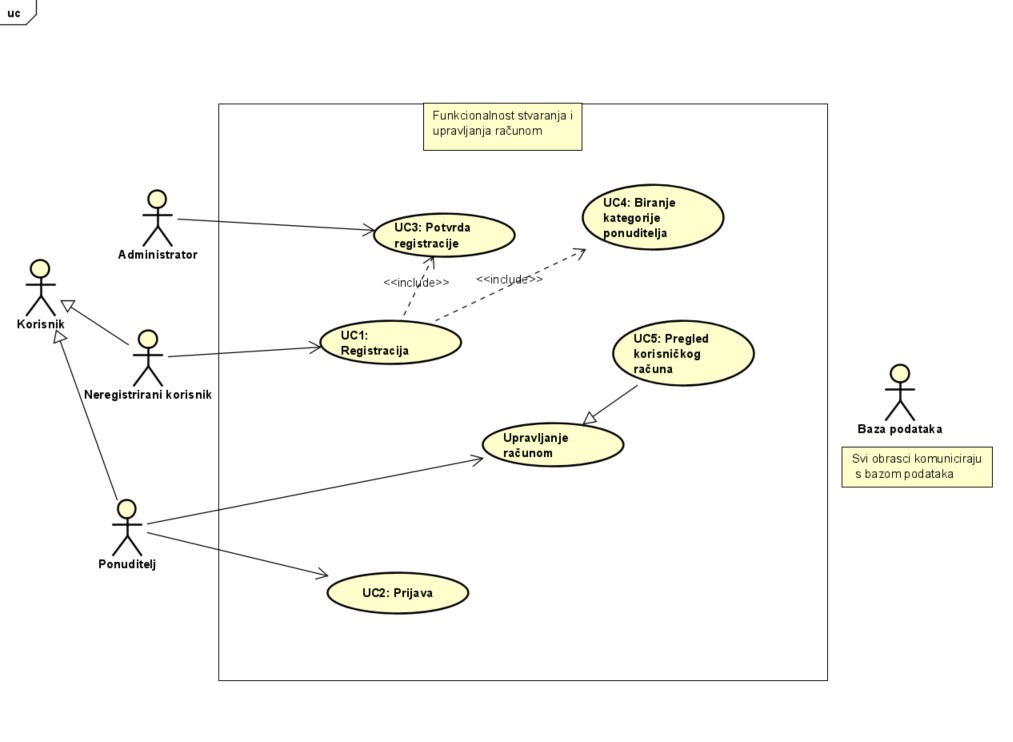
\includegraphics[width = \textwidth]{DO1}
    \caption{Caption}
    \label{fig:enter-label}
\end{figure}

Dijagram obrazaca 2

\begin{figure}
    \centering
    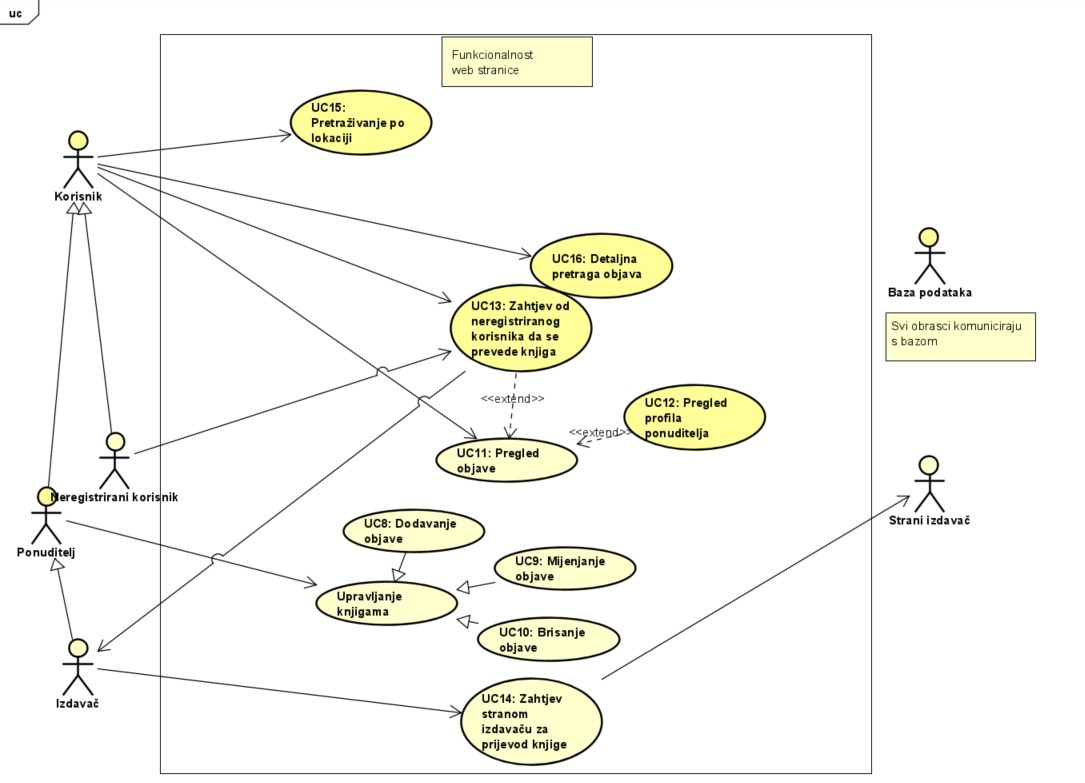
\includegraphics[width = \textwidth]{DO2}
    \caption{Caption}
    \label{fig:enter-label}
\end{figure}
				\eject	
					
				\subsubsection{Dijagrami obrazaca uporabe}
					
					\textit{Prikazati odnos aktora i obrazaca uporabe odgovarajućim UML dijagramom. Nije nužno nacrtati sve na jednom dijagramu. Modelirati po razinama apstrakcije i skupovima srodnih funkcionalnosti.}
				\eject		
				
			\subsection{Sekvencijski dijagrami}
				
				\textbf{\textit{dio 1. revizije}}\\
				
				\textit{Nacrtati sekvencijske dijagrame koji modeliraju najvažnije dijelove sustava (max. 4 dijagrama). Ukoliko postoji nedoumica oko odabira, razjasniti s asistentom. Uz svaki dijagram napisati detaljni opis dijagrama.}
				\eject
	
		\section{Ostali zahtjevi}
		
			\textbf{\textit{dio 1. revizije}}\\
		 
			 \textit{Nefunkcionalni zahtjevi i zahtjevi domene primjene dopunjuju funkcionalne zahtjeve. Oni opisuju \textbf{kako se sustav treba ponašati} i koja \textbf{ograničenja} treba poštivati (performanse, korisničko iskustvo, pouzdanost, standardi kvalitete, sigurnost...). Primjeri takvih zahtjeva u Vašem projektu mogu biti: podržani jezici korisničkog sučelja, vrijeme odziva, najveći mogući podržani broj korisnika, podržane web/mobilne platforme, razina zaštite (protokoli komunikacije, kriptiranje...)... Svaki takav zahtjev potrebno je navesti u jednoj ili dvije rečenice.}
			 
			 
			 
	